\documentclass[12pt]{article}

\usepackage{graphicx}

\title{Evolutionary Mechanics}
\author{Tobias Jacob, Raffaele Guillera, Ali Muddasar}

\begin{document}

\maketitle

\begin{abstract}
    We developed an application that is able to develop mechanical structures using an evolutionary algorithm. This approach can be scaled efficiently across many different nodes.
\end{abstract}

\section{Method}

Our project is divided in two sections and corresponding layers of parallelism. The first one is solving the mechanical equations to check if a mechanical structure can withstand a force. Figure~\ref{fig:Mechanical_Simulation} shows the result of such a simulation. The shape of a figure is approximated through squares.

\begin{figure}[t]
    \centering
    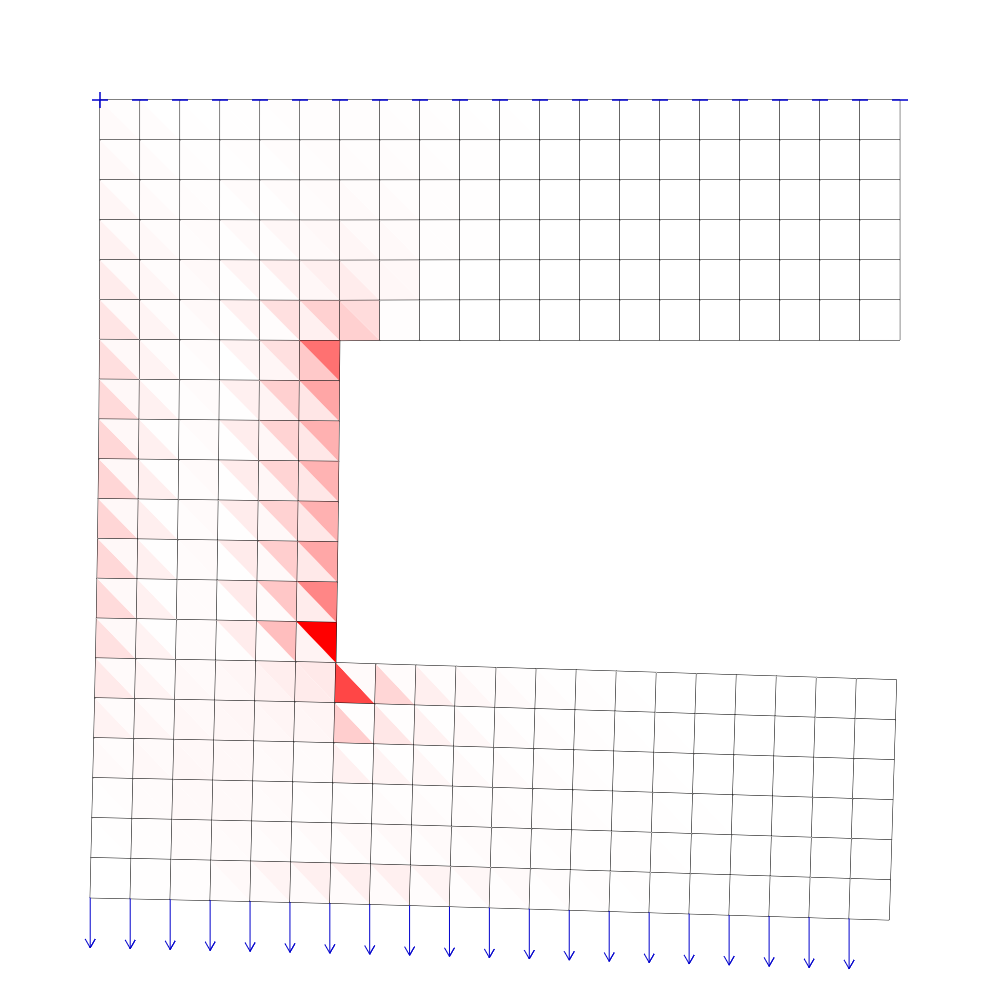
\includegraphics[width=0.8\textwidth]{images/MechaincalStructure.png}
    \caption{Result of a mechanical simulation}
    \label{fig:Mechanical_Simulation}
\end{figure}


The second stage is the evolutionary algorithm. The best 10\% survive in each round. The structures mutate and are simulated again. Even though we put a lot of effort into parallelizing the equation solver, it turned out, that in the end it is faster to parallelize just the evolutionary algorithm instead of parallelizing the evolutionary algorithm and the equation solver. This is, because the core count is usually lower than the generation size, which means that each core can process its own structure. 

\subsection{Speeding up the equation solver}

\texttt{OpenMP} is used for parallelizing the equation solver. The reason for that is the tight coupeling between the data. \texttt{gprof} revealed that the equation solver spends most of it's time in the sparse matrix multiplication, however the whole equation solver class works parallelized.

\begin{itemize}
    \item The equation setup process adds the local element striffness matrix into the global equation system. Depending on the mechanical structure, the position of different planes appears rather random. Therefore, a lock is needed to prevent a race condition. Because the matrix is sparse and each thread works on its own plane, that typically are not directly connected, it is unprobable that two threads operate on the same equation row at the same time. A global lock would introduce an unnecessary penalty, therefore each row uses it's own lock.
    \item All linear algebra operations work in parallel. There are two types of these operations. In Addition, scalar multiplication, matrix multiplication or assigning a constant value, each thread processes its own chunk of rows. This means, that these operations to not require an implicit or explicit barrier. If for example, a vector addtion follows a scalar multiplication, it is fine if the first thread begins with the scalar multiplication before the second thread has finished the vector additon, since each of them operates on its own set of rows.
    
    However, in the conjugate gradient method there are also operations like the scalar product or the norm of the vector. These operations require a reduction and have an implicit barrier.
    \item In the beginning, a unique index has to be assigned to each Plane and corner. This is not parallelizable, as the total number of planes and corners is unkown and does not follow a predictable pattern.
\end{itemize}

The equation solver has theoretically strong scalability, as the dominant part in the computational complexity, the sparse matrix multiplication, can be split accodring to rows. In practice however, there is a significant overhead in creating the threads. This means, that the speedup becomes only notable for problem sizes above 50.

Also, the evolutionary algorithm easily solves several thousand equation systems per second, and for the problem sizes that we evaluated the algorithm on, the thread creation becomes the significant overhead. So while the program is still capable of utilizing multiple cores for solving the equation, we rather decided to let each core process one or multiple structures per generation.

Nevertheless, the Equation Solver is a powerful solver, that scales well with core-count. It is able to solve a mechanical structure that consists of . It also showcases OpenMP and locks well.

\end{document}